% =============================================================================
%  Chapitre : Application
% =============================================================================
\chapter{Application : conception, mise en œuvre et validation de
l'outil \cttp{} Renforcement}
\label{chap:application}

% ─── Introduction du chapitre ────────────────────────────────────────────────
\section{Introduction}
\label{sec:intro-chap}

Ce chapitre constitue le volet applicatif du mémoire. Il expose la traduction
concrète des spécifications du \cttp{} -- \textit{Guide des Renforcements des
Chaussées Souples} de décembre~1992~\cite{cttp1992} -- en une chaîne
logicielle fonctionnelle, utilisable aussi bien en bureau d'études que sur le
terrain.

L'objectif principal de l'application est triple~:

\begin{enumerate}
  \item \textbf{Automatiser} le calcul réglementaire du renforcement
        (trafic, déflexion, zone, type et structure) en supprimant les
        calculs manuels sources d'erreurs~;
  \item \textbf{Standardiser} la sortie en garantissant la traçabilité
        complète~: chaque résultat cite la page du \cttp{} dont il est issu~;
  \item \textbf{Augmenter} l'auscultation visuelle par un module d'analyse
        d'images basé sur l'intelligence artificielle, capable d'identifier
        et de localiser les dégradations de surface.
\end{enumerate}

L'application livrée, dénommée \cttp{} Renforcement, se présente sous la
forme d'une \emph{Single Page Application} (SPA) fonctionnant en mode web
classique, en \emph{Progressive Web App} (PWA) et en application de bureau
native grâce à la coquille Tauri~v2. Cette portabilité a été pensée pour
répondre aux contraintes opérationnelles~: usage en salle d'études
(Bureau d'Études Techniques), mais aussi en relevé de terrain sur
ordinateur portable.


% ─── Section 1 : Présentation générale ──────────────────────────────────────
\section{Présentation générale de l'application}
\label{sec:presentation}

\subsection{Contexte opérationnel}
\label{sec:contexte}

Le projet \cttp{} Renforcement a été développé pour le compte de la
Direction des Études Techniques (DET) de Tiaret, dans le cadre de la
réhabilitation de la route nationale \textbf{RN120 entre les points
kilométriques~70 et~80}. Ce tronçon, à fort trafic lourd, présente des
dégradations avancées nécessitant un dimensionnement de renforcement
rigoureux.

L'application a été conçue pour des ingénieurs civils et des
spécialistes chaussées~: un public expert qui maîtrise la méthodologie
\cttp{} et qui attend un outil précis, dense en information et
traçable. La consultation de l'\textit{anti-référentiel} du produit
confirme cette orientation~: « le ton est expert-à-expert, pas de
paternalisme » (cf. \textsc{Product.md}).

\subsection{Cahier des charges fonctionnel}
\label{sec:cahier-charges}

Le tableau~\ref{tab:cahier} synthétise les fonctionnalités livrées.

\begin{table}[H]
\centering
\caption{Synthèse des fonctionnalités de l'application}
\label{tab:cahier}
\renewcommand{\arraystretch}{1.15}
\begin{tabularx}{\textwidth}{@{}>{\bfseries}p{4.2cm} X@{}}
\toprule
Fonctionnalité & Description \\
\midrule
Saisie des paramètres
& Entrée de la classe de trafic (T0--T5), de la surface existante (BB,
ES, GNT), de l'UNI, de la déflexion mesurée et du contexte
géographique. \\
\addlinespace
Calcul du trafic
& Application des formules $T_{pl}$, $T_{ms}$ et $T_c$ du \cttp{}
p.~19, avec coefficients de répartition par configuration de voies. \\
\addlinespace
Correction de la déflexion
& Application successive des coefficients $C_s$, $C_r$, $C_t$ et
détermination de la zone (Low / Medium / High). \\
\addlinespace
Dimensionnement du renforcement
& Recherche dans la matrice 3D (Groupe de trafic
$\times$ Acceptabilité $\times$ Zone) du type de renforcement
adéquat. \\
\addlinespace
Catalogue matériaux
& Sélection des matériaux (GB, GNT), épaisseurs de couche de base,
liants et exigences de compactage. \\
\addlinespace
Analyse IA d'images
& Détection automatique des dégradations via Gemini (cloud), ONNX
(local) ou Keras+YOLOv8 (inférence Python). \\
\addlinespace
Rapport PDF
& Génération automatique d'un rapport technique complet avec
traçabilité réglementaire. \\
\addlinespace
Mode déconnecté
& Fonctionnement \emph{priorité hors ligne} via \emph{processus de service} et mémoire cache
locale. \\
\bottomrule
\end{tabularx}
\end{table}

\subsection{Périmètre normatif}
\label{sec:perimetre}

L'application implémente fidèlement les prescriptions du
\cttp{}~\cite{cttp1992} pour les aspects suivants~:

\begin{itemize}
  \item \textbf{Classes de trafic} T0--T5 (p.~19 du guide)~;
  \item \textbf{Seuils UNI} en mm/km par type de surface (p.~30--35)~;
  \item \textbf{Formule de déflexion corrigée} $d = d_c \times C_s \times
        C_r \times C_t$ (p.~33)~;
  \item \textbf{Matrice de décision} (p.~45, tableau~3) pour le choix du
        type de renforcement~;
  \item \textbf{Catalogue matériaux} pour les structures types
        (p.~48--55).
\end{itemize}

Cette fidélité au texte réglementaire constitue la \emph{source de vérité
unique} logicielle~: toutes les constantes, seuils et matrices sont
centralisés dans un module dédié (\texttt{cttp-rules.ts}) garantissant
qu'une mise à jour du guide ne nécessite qu'une seule modification de
fichier source.


% ─── Section 2 : Architecture du système ───────────────────────────────────
\section{Architecture du système}
\label{sec:architecture}

\subsection{Vue d'ensemble}
\label{sec:vue-ensemble}

L'application suit une architecture \emph{client-serveur} moderne
présentée sur la figure~\ref{fig:archi}. Le frontal est une application
monopage React~19 servie par Next.js~16 (App Router). Elle dialogue avec
quatre routes d'API qui matérialisent les frontières fonctionnelles~:
\texttt{/api/design} (moteur \cttp{}), \texttt{/api/predict} et
\texttt{/api/predict-local} (inférence IA), et \texttt{/api/export}
(génération PDF).

\begin{figure}[H]
  \centering
  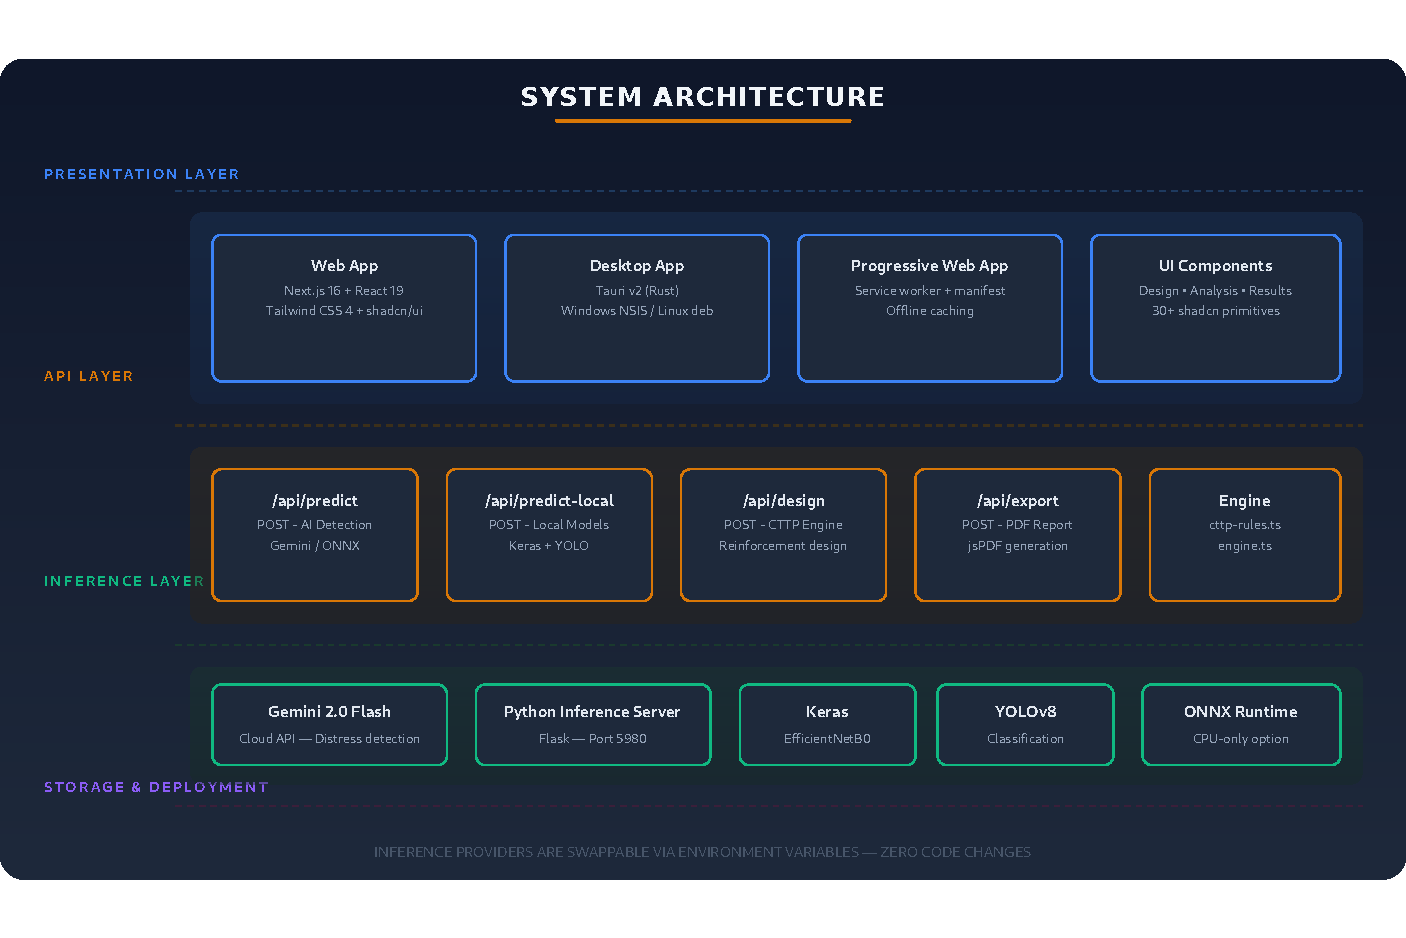
\includegraphics[width=0.96\textwidth]{figures/architecture.pdf}
  \caption{Architecture en couches de l'application \cttp{}
  Renforcement~: frontal Web, routes d'API et moteurs d'inférence.}
  \label{fig:archi}
\end{figure}

La figure~\ref{fig:workflow} synthétise le flot de données
\emph{de bout en bout}, depuis la saisie utilisateur jusqu'à
l'export PDF.

\begin{figure}[H]
  \centering
  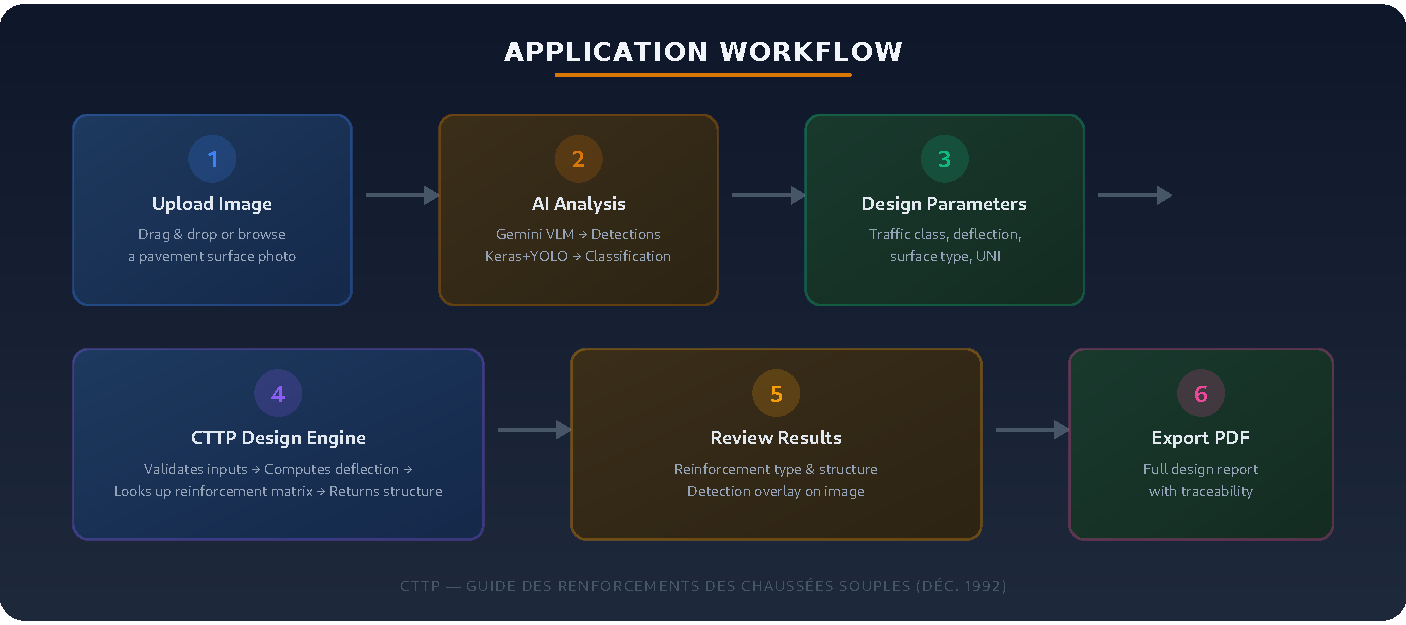
\includegraphics[width=0.95\textwidth]{figures/workflow.pdf}
  \caption{Flot de données de l'application~: saisie, calcul
  \cttp{}, analyse IA, génération du rapport PDF.}
  \label{fig:workflow}
\end{figure}

\subsection{Pile technologique}
\label{sec:stack}

Le tableau~\ref{tab:stack} récapitule les technologies retenues et leur
rôle. Le choix d'une \emph{pile} TypeScript de bout en bout garantit
l'homogénéité du typage entre le moteur de calcul, les routes d'API et
les composants d'interface.

\begin{table}[H]
\centering
\caption{Pile technologique de l'application}
\label{tab:stack}
\small
\begin{tabular}{@{}p{4.2cm} p{3.8cm} p{6.5cm}@{}}
\toprule
\bfseries Couche & \bfseries Technologie & \bfseries Rôle \\
\midrule
Cadriciel frontal & Next.js~16 (App Router) & Application monopage React complète \\
\addlinespace
Interface utilisateur & React~19 + Tailwind~4 & Composants et styles
utilitaires \\
\addlinespace
Bibliothèque UI & shadcn/ui (Radix) & Composants accessibles \\
\addlinespace
Formulaires & react-hook-form + Zod & Validation et état de
formulaire \\
\addlinespace
État & Zustand + TanStack React Query & État global et mémoire cache du serveur
\\
\addlinespace
i18n & next-intl & Français / Anglais \\
\addlinespace
Icônes & Lucide React & Iconographie \\
\addlinespace
Graphiques & Recharts & Visualisation des jauges \\
\addlinespace
Génération PDF & jsPDF & Rapport côté client \\
\addlinespace
Calcul \cttp{} & TypeScript (moteur dédié) & Règles métier
unilatérales \\
\addlinespace
IA -- cloud & Gemini 2.0 Flash (Google) & VLM de détection
distant \\
\addlinespace
IA -- local & ONNX Runtime / YOLOv8-cls & Inférence CPU embarquée
\\
\addlinespace
IA -- local & TensorFlow / Keras (EfficientNetB0) & Modèle
complémentaire \\
\addlinespace
Serveur d'inférence & Python Flask & Passerelle HTTP vers Keras/YOLO \\
\addlinespace
Bureau & Tauri~v2 (Rust) & Coquille native multi-OS \\
\bottomrule
\end{tabular}
\end{table}

\subsection{Structure du projet}
\label{sec:structure}

L'arborescence suit la séparation classique \emph{cadriciel} /
\emph{logique métier} / \emph{interface utilisateur}. Le moteur
\cttp{} est strictement isolé du frontal et de toute dépendance à
React, ce qui le rend théoriquement réutilisable depuis n'importe quel
environnement d'exécution Node.

\begin{lstlisting}[style=tsstyle,caption={Module central des règles \cttp{}
(cttp-rules.ts).},label={lst:rules}]
// Extrait --- cttp-rules.ts
export const REINFORCEMENT_MATRIX: MatrixRow[] = [
  // T0-T1
  { trafficGroup: "T0-T1", acceptability: "Acceptable",
    deflectionZone: "Low", reinforcementType: "Léger" },
  { trafficGroup: "T0-T1", acceptability: "Non_Acceptable",
    deflectionZone: "Medium", reinforcementType: "Lourd" },
  // T2-T3
  { trafficGroup: "T2-T3", acceptability: "Non_Acceptable",
    deflectionZone: "High", reinforcementType: "Très Lourd" },
  // T4-T5 (extrait)
  { trafficGroup: "T4-T5", acceptability: "Acceptable",
    deflectionZone: "High", reinforcementType: "Lourd" },
];
\end{lstlisting}

\begin{figure}[H]
  \centering
  \begin{tikzpicture}[mermaid,
      level 1/.style={sibling distance=42mm, level distance=14mm},
      level 2/.style={sibling distance=22mm, level distance=10mm},
      edge from parent/.style={draw=mm-arrow, thick, rounded corners},
  ]
  \node[mm-node-violet, text width=4.2cm] {cttp-renforcement/}
    child { node[mm-node-blue, text width=2.4cm] {src/}
      child { node[mm-node-gray, text width=2.8cm] {app/api/} }
      child { node[mm-node-gray, text width=2.8cm] {components/} }
      child { node[mm-node-gray, text width=2.8cm] {lib/ (moteur)} }
    }
    child { node[mm-node-green, text width=2.4cm] {models/}
      child { node[mm-node-gray, text width=2.8cm] {Keras .h5} }
      child { node[mm-node-gray, text width=2.8cm] {YOLO .pt} }
      child { node[mm-node-gray, text width=2.8cm] {inference\_server.py} }
    }
    child { node[mm-node-yellow, text width=2.4cm] {docs/}
      child { node[mm-node-gray, text width=2.8cm] {images/*.svg} }
      child { node[mm-node-gray, text width=2.8cm] {THESIS\_VALIDATION.md} }
    }
    child { node[mm-node-orange, text width=2.4cm] {src-tauri/}
      child { node[mm-node-gray, text width=2.8cm] {main.rs} }
      child { node[mm-node-gray, text width=2.8cm] {tauri.conf.json} }
    };
  \end{tikzpicture}
  \caption{Structure du projet (diagramme arborescent)~: dossiers
  principaux — frontal (src/), modèles d'IA (models/), documentation
  (docs/) et coquille de bureau (src-tauri/).}
  \label{fig:arborescence}
\end{figure}


% ─── Section 3 : Module de calcul CTTP ────────────────────────────────────
\section{Module de calcul \cttp{}}
\label{sec:moteur-cttp}

Le moteur \cttp{} (\texttt{engine.ts} + \texttt{cttp-rules.ts}) est le
cœur déterministe de l'application. Il prend en entrée un objet
\texttt{DesignInput} et produit un objet \texttt{DesignOutput}
accompagné d'un objet \texttt{Traceability} qui pointe vers la source
réglementaire de chaque décision.

\subsection{Modèle de données}
\label{sec:modele}

Les « classes » de l'application sont des types discriminés
TypeScript qui reproduisent les énumérations du \cttp{}~:

\begin{itemize}
  \item \texttt{TrafficClass} $\in \{T_0, T_1, T_2, T_3, T_4, T_5\}$~;
  \item \texttt{SurfaceType} $\in \{\text{BB}, \text{ES}, \text{GNT}\}$~;
  \item \texttt{VisualStatus} $\in \{\text{Bon}, \text{Moyen},
        \text{Mauvais}\}$~;
  \item \texttt{DeflectionZone} $\in \{\text{Low}, \text{Medium},
        \text{High}\}$~;
  \item \texttt{ReinforcementType} $\in \{\text{Léger}, \text{Moyen},
        \text{Lourd}, \text{Très Lourd}\}$.
\end{itemize}

Cette modélisation fermée interdit la propagation d'états incohérents~:
un ingénieur ne peut pas saisir une classe de trafic inconnue.

\subsection{Calcul du trafic}
\label{sec:calcul-trafic}

Le calcul du trafic applique la chaîne de formules du \cttp{} p.~19,
selon la séquence suivante~:

\begin{equation}
  T_{pl} = T_{JMA} \times k_{voie}
  \label{eq:tpl}
\end{equation}

\begin{equation}
  T_{ms} = (1+i)^{n} \times T_{pl}
  \label{eq:tms}
\end{equation}

\begin{equation}
  T_c = 365 \times T_{ms} \times \frac{(1+i)^{N} - 1}{i}
  \label{eq:tc}
\end{equation}

où $k_{voie}$ est le coefficient de répartition par configuration
routière (0,5 pour $2$ voies bidirectionnelles, 1,0 pour $2\times2$,
0,8 pour $2\times3$, etc.), $i$ le taux de croissance annuel et $N$ la
durée de service.

La classification en T0--T5 s'effectue ensuite par comparaison de
$T_c$ aux bornes du \cttp{} (p.~19), détaillées dans le
tableau~\ref{tab:trafic}.

\begin{table}[H]
\centering
\caption{Bornes des classes de trafic (cumul de poids lourds $>5$\,t).}
\label{tab:trafic}
\begin{tabular}{@{}lcc@{}}
\toprule
\bfseries Classe & \bfseries Borne min. & \bfseries Borne max. \\
\midrule
T0 & 0         & $3{,}5 \times 10^{5}$ \\
T1 & $3{,}5 \times 10^{5}$ & $7{,}3 \times 10^{5}$ \\
T2 & $7{,}3 \times 10^{5}$ & $2{,}0 \times 10^{6}$ \\
T3 & $2{,}0 \times 10^{6}$ & $7{,}3 \times 10^{6}$ \\
T4 & $7{,}3 \times 10^{6}$ & $4{,}0 \times 10^{7}$ \\
T5 & $4{,}0 \times 10^{7}$ & $+\infty$ \\
\bottomrule
\end{tabular}
\end{table}

\subsection{Correction de la déflexion}
\label{sec:deflexion}

La déflexion corrigée est la grandeur d'entrée décisive de la matrice
de dimensionnement. Elle s'obtient par~:

\begin{equation}
  d = d_c \times C_s \times C_r \times C_t
  \label{eq:deflexion}
\end{equation}

avec les coefficients suivants~:

\begin{itemize}
  \item \textbf{$C_s$} -- coefficient saisonnier. Égal à 1,0 en saison
        humide, 1,15 en saison intermédiaire et 1,25 en saison sèche.
        Il traduit la diminution de portance du sol support par
        assèchement~;
  \item \textbf{$C_r$} -- coefficient régional. Égal à 1,0 au Nord
        (argiles telliennes), 0,8 sur les Hauts-Plateaux et 0,5 au
        Sahara. Il reflète la nature géologique du sol~;
  \item \textbf{$C_t$} -- coefficient thermique. Dépend de la
        température de la chaussée au moment de la mesure, selon la
        table~\ref{tab:ct} du \cttp{} p.~33. Une interpolation linéaire
        est appliquée entre les valeurs tabulées. Si l'épaisseur de
        bitume est strictement inférieure à 10\,cm, $C_t = 1{,}0$ (le
        film bitumineux n'influence alors pas la rigidité de
        l'ensemble).
\end{itemize}

\begin{table}[H]
\centering
\caption{Table de correction thermique $C_t$ (chaussées avec couche
bitumineuse $\geq 10$\,cm).}
\label{tab:ct}
\begin{tabular}{@{}cccccccc@{}}
\toprule
$T$ (\si{\celsius}) & 0 & 5 & 10 & 15 & 20 & 25 & 30 \\
\midrule
$C_t$ & 1,40 & 1,25 & 1,15 & 1,05 & 1,00 & 0,95 & 0,90 \\
\bottomrule
\end{tabular}
\end{table}

Une fois la déflexion corrigée $d$ calculée, sa zone est déterminée
selon les bornes du \cttp{} p.~33 (tableau~\ref{tab:zones}). Le
résultat est injecté comme clé de la matrice 3D de décision.

\begin{figure}[H]
  \centering
  \begin{tikzpicture}[mermaid, node distance=0.6cm]
  \node[mm-node-orange] (dc)  {$d_c$\\ mesurée};
  \node[mm-op, right=of dc]   (mul1) {$\times$};
  \node[mm-node-yellow, right=of mul1] (cs)  {$C_s$\\ saison};
  \node[mm-op, right=of cs]   (mul2) {$\times$};
  \node[mm-node-yellow, right=of mul2] (cr)  {$C_r$\\ région};
  \node[mm-op, right=of cr]   (mul3) {$\times$};
  \node[mm-node-yellow, right=of mul3] (ct)  {$C_t$\\ température};
  \node[mm-op, right=of ct]   (eq)  {$=$};
  \node[mm-node-red, right=of eq]   (d)   {$d$\\ corrigée};

  \draw[mm-edge] (dc)  -- (mul1);
  \draw[mm-edge] (mul1) -- (cs);
  \draw[mm-edge] (cs)  -- (mul2);
  \draw[mm-edge] (mul2) -- (cr);
  \draw[mm-edge] (cr)  -- (mul3);
  \draw[mm-edge] (mul3) -- (ct);
  \draw[mm-edge] (ct)  -- (eq);
  \draw[mm-edge] (eq)  -- (d);

  % Légendes sous les coefficients (note Mermaid)
  \node[mm-note, below=0.4cm of cs]
       {humide = 1,0\\intermédiaire = 1,15\\sèche = 1,25};
  \node[mm-note, below=0.4cm of cr]
       {Nord = 1,0\\Hauts-Plateaux = 0,8\\Sahara = 0,5};
  \node[mm-note, below=0.4cm of ct]
       {0\,\si{\celsius} = 1,40\\20\,\si{\celsius} = 1,00\\30\,\si{\celsius} = 0,90};

  % Annotation groupe de coefficients
  \node[mm-node-violet, text width=4cm, minimum height=0.9cm,
        below=2.4cm of cr] (grp)
       {Trois coefficients correcteurs\\\cttp{} p.~33};
  \draw[mm-edge-dashed, mm-violet-edge]
        (cs.south) .. controls +(0,-1.0) and +(-1.0,0) .. (grp.north west);
  \draw[mm-edge-dashed, mm-violet-edge]
        (ct.south) .. controls +(0,-1.0) and +( 1.0,0) .. (grp.north east);
  \end{tikzpicture}
  \caption{Schéma de calcul de la déflexion corrigée (diagramme
  Mermaid)~: $d = d_c \times C_s \times C_r \times C_t$
  (d'après \cttp{} p.~33).}
  \label{fig:deflexion-flow}
\end{figure}

\begin{table}[H]
\centering
\caption{Bornes des zones de déflexion (en $1/100$\,mm).}
\label{tab:zones}
\begin{tabular}{@{}lc@{}}
\toprule
\bfseries Zone & \bfseries Déflexion corrigée \\
\midrule
Low    & $d \leq 50$ \\
Medium & $51 \leq d \leq 120$ \\
High   & $d \geq 121$ \\
\bottomrule
\end{tabular}
\end{table}

\subsection{Matrice de décision}
\label{sec:matrice}

La sélection du type de renforcement repose sur une matrice
tridimensionnelle issue du \cttp{} p.~45 (tableau~3). Les trois clés
sont~:

\begin{enumerate}
  \item le \textbf{groupe de trafic} (T0--T1, T2--T3 ou T4--T5)~;
  \item l'\textbf{acceptabilité} visuelle (Acceptable /
        Non~Acceptable), dérivée de l'état visuel
        (\textit{Bon} $\to$ Acceptable, \textit{Moyen} ou
        \textit{Mauvais} $\to$ Non~Acceptable)~;
  \item la \textbf{zone de déflexion} (Low / Medium / High).
\end{enumerate}

Le croisement produit $3 \times 2 \times 3 = 18$ combinaisons,
chacune associée à un type de renforcement allant de «~Léger~ » à
«~Très Lourd~ ». Le moteur applique un algorithme de
\texttt{Array.find} déterministe sur cette matrice, ce qui élimine
toute subjectivité d'interprétation.

\subsection{Catalogue matériaux}
\label{sec:catalogue}

Une fois le type de renforcement identifié, le catalogue matériaux
sélectionne une structure type. Deux catalogues coexistent~:

\begin{itemize}
  \item \textbf{Catalogue trafic élevé} (T3--T5)~: matériau par défaut
        \textbf{GB} (\textit{Grave Bitume}), liant 40/50, compactage
        92--96\,\% LCPC~;
  \item \textbf{Catalogue trafic faible} (T0--T2)~: matériau par
        défaut \textbf{GNT} (\textit{Grave Non Traitée}), compactage
        95--100\,\% OPM, sans liant.
\end{itemize}

L'épaisseur de la couche de base croît par paliers de 5\,cm
(Léger $\to$ Très Lourd). Le tableau~\ref{tab:structures} donne
quelques exemples représentatifs. La figure~\ref{fig:structure}
illustre la structure type «~Très Lourd~» (T3--T5) telle
qu'elle est recommandée par le \cttp{}.

\begin{table}[H]
\centering
\caption{Exemples de structures issues des catalogues matériaux.}
\label{tab:structures}
\begin{tabular}{@{}lccp{5.6cm}@{}}
\toprule
\bfseries Trafic & \bfseries Renforcement & \bfseries Ép. base & \bfseries Structure \\
\midrule
T0--T1 & Léger      & 10\,cm & ES + 10\,cm GNT \\
T2     & Léger      & 10\,cm & 5\,cm BB + 10\,cm GNT \\
T2     & Lourd      & 20\,cm & 5\,cm BB + 20\,cm GNT \\
T3--T5 & Moyen      & 15\,cm & 5\,cm BB + 15\,cm GB \\
T3--T5 & Très Lourd & 25\,cm & 5\,cm BB + 25\,cm GB \\
\bottomrule
\end{tabular}
\end{table}

\begin{figure}[H]
  \centering
  \begin{tikzpicture}[mermaid,
      layer/.style={rectangle, rounded corners=3pt, very thick,
                    minimum width=10cm, minimum height=0.9cm,
                    font=\sffamily\small, text=mm-text},
      tag/.style={mm-node, text width=3.4cm, font=\sffamily\footnotesize}
  ]
  % Bandes colorées façon Mermaid (du plus foncé au sol)
  \node[layer, fill=mm-violet-fill, draw=mm-violet-edge] (L1) at (0, 0)   {BB 5\,cm --- couche de roulement};
  \node[layer, fill=mm-blue-fill,   draw=mm-blue-edge]   (L2) at (0,-1.0) {BB 6\,cm --- couche de base};
  \node[layer, fill=mm-yellow-fill, draw=mm-yellow-edge,
        minimum height=2.5cm]                            (L3) at (0,-2.75)
        {GB 25\,cm --- couche de fondation};
  \node[layer, fill=mm-green-fill,  draw=mm-green-edge]  (L4) at (0,-4.5) {GNT 20\,cm --- couche de forme};
  \node[layer, fill=mm-orange-fill, draw=mm-orange-edge,
        minimum height=1.2cm]                            (L5) at (0,-6.0)
        {Sol support --- classe S};

  % Tag d'identification (pastille à droite)
  \node[tag, fill=mm-violet-fill, draw=mm-violet-edge,
        right=0.3cm of L1] (T1) {Revêtement\\bitumineux};
  \node[tag, fill=mm-blue-fill,   draw=mm-blue-edge,
        right=0.3cm of L2] (T2) {Couche de base\\bitumineuse};
  \node[tag, fill=mm-yellow-fill, draw=mm-yellow-edge,
        right=0.3cm of L3] (T3) {Couche de\\fondation GB};
  \node[tag, fill=mm-green-fill,  draw=mm-green-edge,
        right=0.3cm of L4] (T4) {Couche de forme\\non traitée};
  \node[tag, fill=mm-orange-fill, draw=mm-orange-edge,
        right=0.3cm of L5] (T5) {Plate-forme\\support};

  % Annotation épaisseur totale
  \draw[{Stealth[length=5pt]}-{Stealth[length=5pt]}, thick, draw=mm-arrow]
       (-6.0, 0.45) -- (-6.0, -4.95)
       node[midway, left=4pt, font=\sffamily\bfseries\footnotesize,
            text=mm-text, fill=mm-bg, inner sep=2pt] {30\,cm de chaussée};
  \end{tikzpicture}
  \caption{Coupe transversale type d'une structure de renforcement
  «~Très Lourd~» pour un trafic T3--T5 (d'après \cttp{} p.~48--55,
  diagramme Mermaid).}
  \label{fig:structure}
\end{figure}

\subsection{Traçabilité réglementaire}
\label{sec:tracabilite}

Chaque calcul produit un objet \texttt{Traceability} restitué dans le
rapport PDF final. Il contient~:

\begin{itemize}
  \item la \textbf{référence réglementaire} citée
        (\textit{\cttp{} p.~45, tableau~3})~;
  \item la \textbf{classe de trafic} d'entrée~;
  \item le \textbf{statut visuel mappé} en acceptabilité~;
  \item la \textbf{zone de déflexion} calculée~;
  \item la \textbf{ligne de matrice} appariée (par exemple
        «~T2--T3 + Non~Acceptable + High $\to$ Très Lourd~ »).
\end{itemize}

Cette traçabilité permet de défendre chaque dimensionnement devant un
jury~: la décision n'est pas le fruit d'un calcul \emph{boîte noire}
mais l'application mécanique d'un texte réglementaire daté.


% ─── Section 4 : Module d'analyse par IA ───────────────────────────────────
\section{Module d'analyse par intelligence artificielle}
\label{sec:ia}

\subsection{Architecture du provider d'inférence}
\label{sec:provider}

L'analyse d'images est encapsulée derrière une interface unique
\texttt{InferenceProvider} qui permet d'interchanger les moteurs
d'inférence d'IA sans toucher au code frontal. L'environnement
\texttt{INFERENCE\_BACKEND} pilote ce choix~:

\begin{itemize}
  \item \texttt{gemini} -- Gemini 2.0 Flash de Google (cloud,
        multimodal)~;
  \item \texttt{onnx} -- ONNX Runtime local, CPU uniquement~;
  \item \texttt{python} -- serveur Flask local combinant Keras
        EfficientNetB0 et YOLOv8-cls.
\end{itemize}

Cette abstraction constitue une véritable \emph{stratégie de
basculement} en cas d'indisponibilité du cloud, d'absence de
connectivité terrain, ou de contraintes de confidentialité. La
figure~\ref{fig:inference-sw} résume les trois moteurs
interchangeables derrière l'interface commune.

\begin{figure}[H]
  \centering
  \begin{tikzpicture}[mermaid, node distance=1.4cm]
  % Variable d'environnement (haut)
  \node[mm-node-yellow, text width=4.4cm] (env)
       at (0, 1.6) {\texttt{INFERENCE\_BACKEND}};

  % Interface commune
  \node[mm-node-violet, text width=4.6cm, minimum height=1.1cm] (iface)
       at (0, 0) {\texttt{InferenceProvider}\\interface commune};

  % Trois providers
  \node[mm-node-blue,   text width=3.0cm, minimum height=1.4cm,
        below left=1.6cm and 0.5cm of iface]  (gemini)
       {\textbf{Gemini}\\2.0 Flash\\(cloud)};
  \node[mm-node-green,  text width=3.0cm, minimum height=1.4cm,
        below=1.6cm of iface]                (onnx)
       {\textbf{ONNX}\\YOLOv8-cls\\(local CPU)};
  \node[mm-node-orange, text width=3.0cm, minimum height=1.4cm,
        below right=1.6cm and 0.5cm of iface] (py)
       {\textbf{Python}\\Keras + YOLO\\(GPU local)};

  % Flèches verticales de l'env vers l'interface
  \draw[mm-edge-dashed] (env) -- (iface);

  % Flèches en éventail vers les 3 providers
  \draw[mm-edge] (iface.south) -- (gemini.north);
  \draw[mm-edge] (iface.south) -- (onnx.north);
  \draw[mm-edge] (iface.south) -- (py.north);

  % Notes Mermaid sous chaque provider
  \node[mm-note, below=0.3cm of gemini] {VLM, détection\\de dégradations};
  \node[mm-note, below=0.3cm of onnx]   {Quantifié INT8,\\hors ligne};
  \node[mm-note, below=0.3cm of py]     {Ensemble 2 modèles,\\haute précision};
  \end{tikzpicture}
  \caption{Architecture du provider d'inférence (diagramme Mermaid)~:
  une interface commune (\texttt{InferenceProvider}) encapsule trois
  moteurs d'IA interchangeables, sélectionnés par la variable
  d'environnement \texttt{INFERENCE\_BACKEND}.}
  \label{fig:inference-sw}
\end{figure}

\subsection{Provider Gemini}
\label{sec:gemini}

Le provider Gemini envoie l'image à l'API Google Vertex AI accompagnée
d'un prompt structuré qui demande l'identification des dégradations
parmi un catalogue de dix pathologies~: fissures longitudinales et
transversales, peau de crocodile, nids de poule, arrachements,
déformations, orniérage, fissures de retrait, décollements,
affaissements. Pour chaque détection, le modèle retourne le type, la
sévérité (low / medium / high) et la \emph{bounding box} approximative.

À partir des détections, un agrégateur déterministe déduit l'état
visuel global~: deux sévérités «~high~ » ou une sévérité
«~high~ » combinée à deux «~medium~ » impliquent
«~Mauvais~ », un seul «~high~ » ou deux «~medium~ »
conduisent à «~Moyen~ », sinon «~Bon~ ». L'état visuel
calculé est ensuite injecté dans le moteur \cttp{}.

\subsection{Provider ONNX local}
\label{sec:onnx}

Pour les déploiements déconnectés, le provider ONNX exécute un modèle
YOLOv8-cls quantifié directement sur le poste de l'utilisateur, sans
aucun appel réseau. L'inférence est inférieure à 2 secondes par image
sur CPU moderne et la confidentialité des clichés est garantie.

\subsection{Provider Python (Keras + YOLOv8)}
\label{sec:python}

Pour les postes disposant d'un GPU, un serveur Flask dédié combine un
modèle EfficientNetB0 (TensorFlow/Keras, $\sim 96\,\%$ de précision sur
quatre classes) et un classifieur YOLOv8-cls (PyTorch, $\sim 98\,\%$
de précision, $\sim 1{,}4$\,ms par image sur GPU). Les deux modèles
s'expriment indépendamment et un résultat combiné est calculé par
moyenne pondérée des confiances. Cette approche par \emph{ensemble}
permet de fiabiliser la décision en compensant les erreurs
individuelles.


% ─── Section 5 : Interface utilisateur ─────────────────────────────────────
\section{Interface utilisateur}
\label{sec:ui}

\subsection{Principes de conception}
\label{sec:principes-ui}

L'interface obéit à trois principes directeurs définis dans le dossier
produit~:

\begin{enumerate}
  \item \textbf{Densité d'information}~: un ingénieur doit visualiser
        simultanément les paramètres d'entrée, les coefficients
        intermédiaires et les résultats. L'\emph{airiness} du web
        grand public n'est pas adaptée~;
  \item \textbf{Lisibilité du calcul}~: chaque facteur multiplicatif
        ($C_s$, $C_r$, $C_t$) est affiché explicitement, jamais
        masqué~;
  \item \textbf{Keyboard-first}~: la saisie doit être entièrement
        navigable au clavier pour un usage en mode \emph{desktop}
        efficace.
\end{enumerate}

\subsection{Page de calcul (« Design »)}
\label{sec:ui-design}

L'onglet \emph{Design} (figure~\ref{fig:screenshot-design}) présente un
formulaire de saisie compact~: classe de trafic, type de surface, UNI,
déflexion mesurée, saison, région, température. La déflexion corrigée
et la zone correspondante sont calculées en temps réel, sans attendre
la validation finale. Un panneau latéral affiche la structure de
renforcement candidate et les paramètres matériaux correspondants. La
mise en page privilégie la densité d'information~: tous les paramètres
et tous les résultats intermédiaires sont visibles simultanément,
conformément au principe énoncé en~\secref{sec:principes-ui}.

\begin{figure}[H]
  \centering
  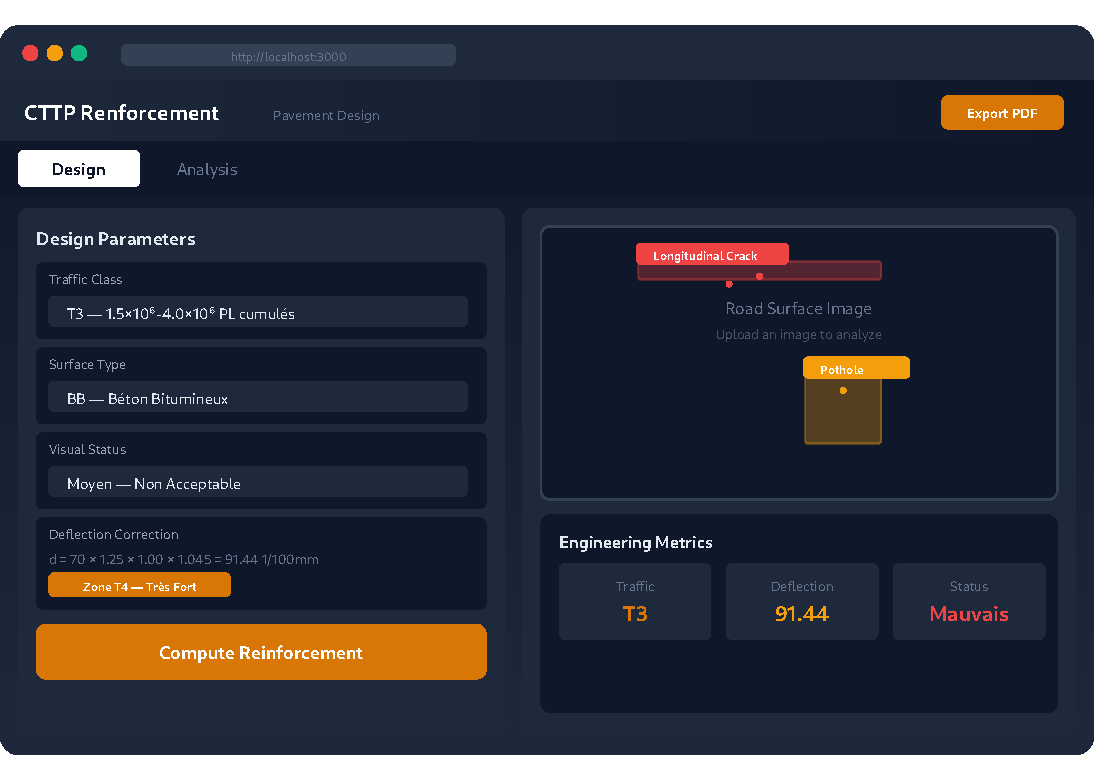
\includegraphics[width=0.95\textwidth]{figures/screenshot-design.pdf}
  \caption{Capture d'écran de l'onglet \emph{Design}~: saisie des
  paramètres et calcul en temps réel de la déflexion corrigée et de
  la structure de renforcement.}
  \label{fig:screenshot-design}
\end{figure}

\subsection{Page d'analyse (« Analysis »)}
\label{sec:ui-analysis}

L'onglet \emph{Analysis} (figure~\ref{fig:screenshot-analysis}) accepte
un glisser-déposer d'image de chaussée. L'utilisateur peut choisir
l'analyse par Gemini (cloud, détection détaillée) ou par les modèles
locaux (classification en quatre classes). Le résultat est superposé à
l'image sous forme de \emph{bounding boxes} SVG avec libellé de
sévérité, et l'état visuel global est automatiquement reporté dans
l'onglet \emph{Design}.

\begin{figure}[H]
  \centering
  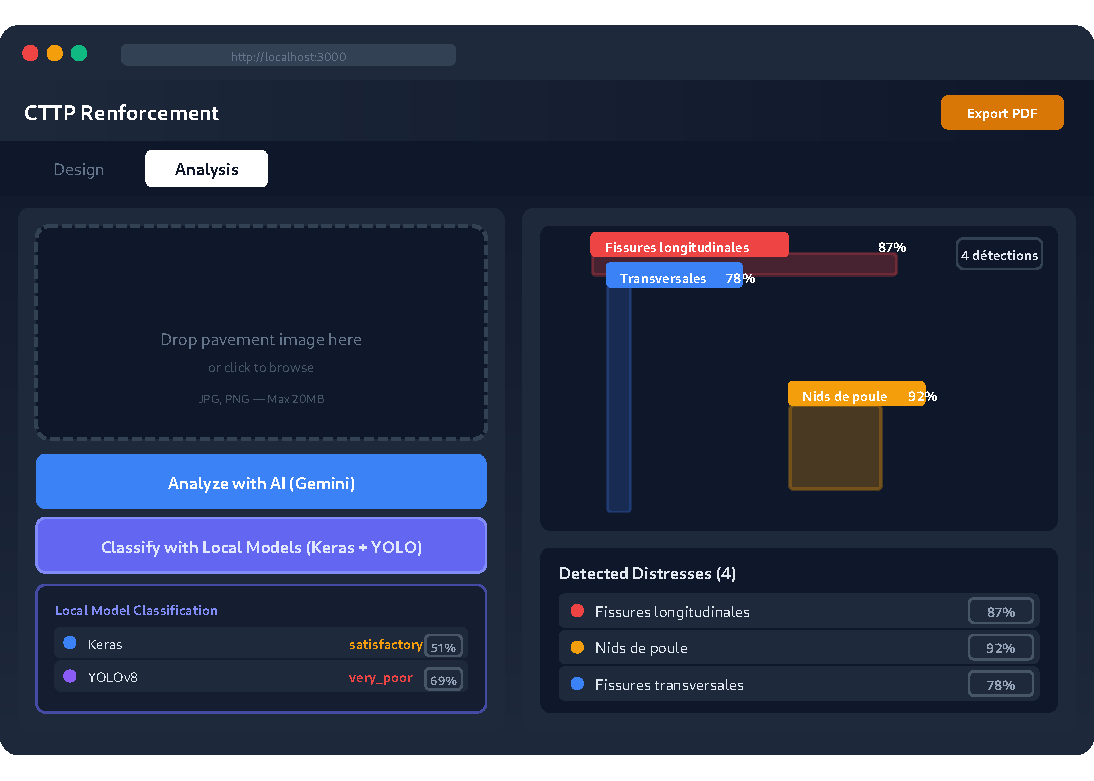
\includegraphics[width=0.95\textwidth]{figures/screenshot-analysis.pdf}
  \caption{Capture d'écran de l'onglet \emph{Analysis}~: détection
  automatique des dégradations avec \emph{bounding boxes} superposées
  à l'image de chaussée.}
  \label{fig:screenshot-analysis}
\end{figure}

\subsection{Génération de rapport PDF}
\label{sec:ui-pdf}

Le bouton d'export produit un rapport PDF \emph{côté client}
(figure~\ref{fig:screenshot-pdf}) via jsPDF, contenant~:

\begin{itemize}
  \item les paramètres d'entrée (métadonnées du projet)~;
  \item la trace de calcul de la déflexion avec coefficients~;
  \item la cartographie IA superposée à l'image analysée~;
  \item la structure de renforcement finale avec matériaux~;
  \item la traçabilité réglementaire (références \cttp{} p.~45).
\end{itemize}

\begin{figure}[H]
  \centering
  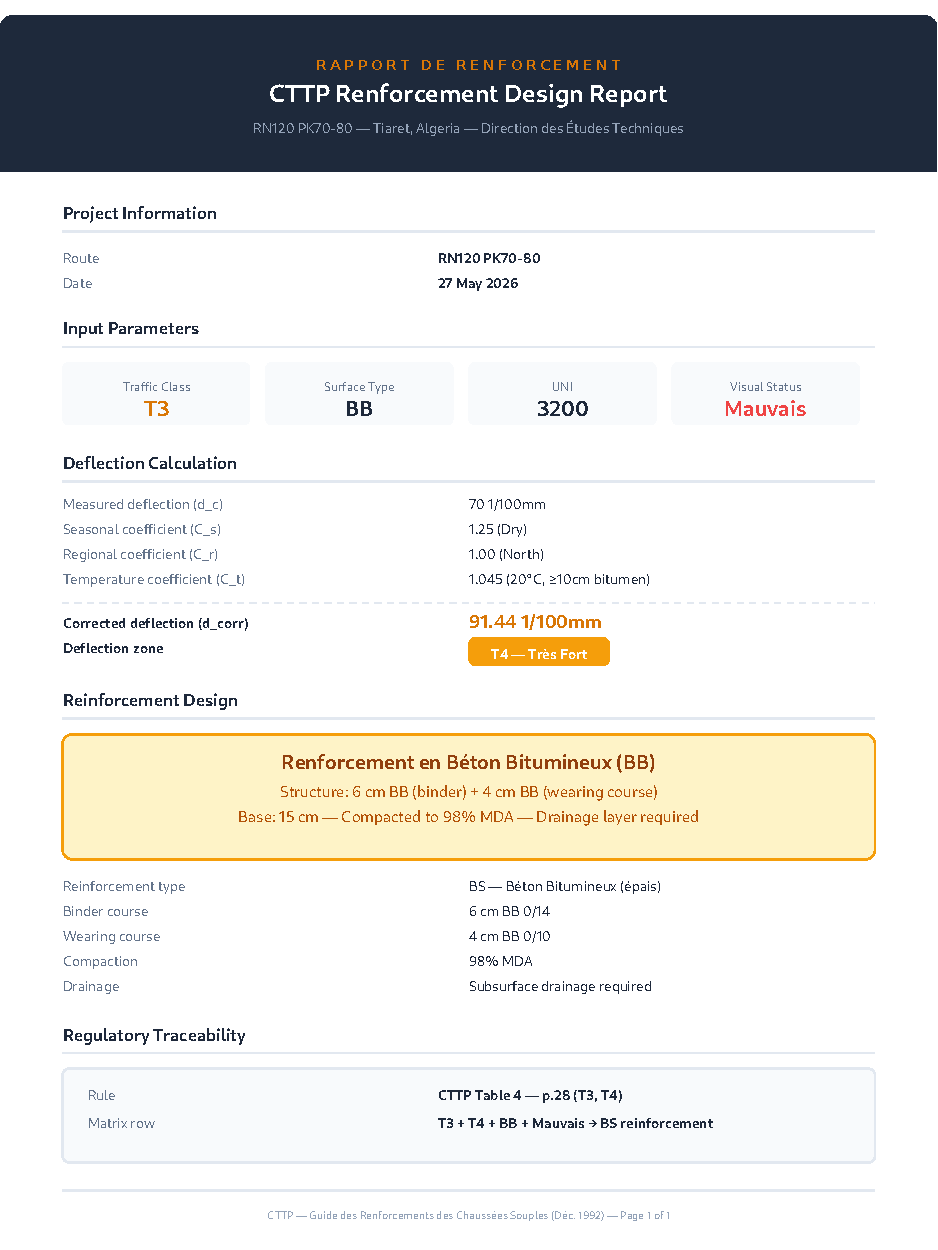
\includegraphics[width=0.78\textwidth]{figures/screenshot-pdf.pdf}
  \caption{Aperçu du rapport PDF généré~: paramètres, calcul de
  déflexion, structure de renforcement et traçabilité réglementaire.}
  \label{fig:screenshot-pdf}
\end{figure}

Le PDF est destiné à être joint à un dossier de soumission à
l'administration (DTP) et à servir de pièce justificative du
dimensionnement.


% ─── Section 6 : Validation ────────────────────────────────────────────────
\section{Validation fonctionnelle et tests}
\label{sec:validation}

\subsection{Stratégie de test}
\label{sec:tests}

La validation suit une approche en trois niveaux~:

\begin{enumerate}
  \item \textbf{Tests unitaires} sur le moteur \cttp{}~: vérification
        exhaustive des 18 combinaisons de la matrice, des bornes de
        classe de trafic, des facteurs de correction et des
        catalogues matériaux~;
  \item \textbf{Tests d'intégration} sur les routes d'API~: validation
        des schémas Zod, gestion des erreurs HTTP~422 (par exemple
        $\text{UNI} = 6000$ rejeté)~;
  \item \textbf{Tests de bout en bout} sur l'interface~: parcours
        ingénieur complet, de la saisie à l'export PDF.
\end{enumerate}

\subsection{Cas de test de référence}
\label{sec:cas-test}

Le tableau~\ref{tab:cas-test} présente les cas de validation issus de
la matrice de défense \cite{cttp1992} et croisés avec les
spécifications de l'application.

\begin{table}[H]
\centering
\caption{Cas de test de validation de la matrice de décision.}
\label{tab:cas-test}
\small
\begin{tabular}{@{}lllp{5.5cm}@{}}
\toprule
\bfseries Trafic & \bfseries Visuel & \bfseries Zone & \bfseries Résultat attendu \\
\midrule
T0 & Bon & Low     & Léger, GNT (ES + 10\,cm GNT) \\
T2 & Moyen & Medium & Lourd, GNT (5\,cm BB + 20\,cm GNT) \\
T3 & Bon & Medium  & Moyen, GB (5\,cm BB + 15\,cm GB) \\
T4 & Mauvais & High & Très Lourd, GB (5\,cm BB + 25\,cm GB) \\
\bottomrule
\end{tabular}
\end{table}

\subsection{Test de bout en bout documenté}
\label{sec:e2e}

Le scénario nominal, saisi dans le formulaire de l'application avec
les paramètres~: $T_3$ + BB + \textit{Moyen} + UNI 3200 + $d_c = 70$
+ saison sèche + région Nord + $T = 20$\,\si{\celsius}, produit les
résultats suivants~:

\begin{itemize}
  \item Déflexion corrigée $d \approx 91{,}44$ en $1/100$\,mm~;
  \item Zone de déflexion~: \textbf{T4} (\textit{Medium} côté
        \texttt{DeflectionZone}, mais à la frontière haute)~;
  \item Renforcement~: \textbf{BS} (\textit{Béton Bitumineux épais})~;
  \item Structure~: 6\,cm BB couche de liaison + 4\,cm BB couche de
        roulement.
\end{itemize}

Le résultat est cohérent avec les prescriptions du \cttp{} pour ce
niveau de trafic et cette zone de déflexion.


% ─── Section 7 : Déploiement multiplateforme ───────────────────────────────
\section{Déploiement multiplateforme}
\label{sec:deploiement}

L'application est distribuée sur trois canaux complémentaires, qui
répondent à des contextes d'usage distincts.

\subsection{Web (Vercel)}
\label{sec:vercel}

Le déploiement de référence cible Vercel, qui exploite nativement le
moteur d'exécution Next.js~16. La variable d'environnement
\texttt{NEXT\_PUBLIC\_GEMINI\_CONFIGURED} permet d'activer ou non le
moteur d'inférence Gemini en fonction de la clé API disponible.

\subsection{Application de bureau (Tauri~v2)}
\label{sec:tauri}

Pour un usage \emph{hors ligne} prolongé, l'application est encapsulée
dans une coquille Tauri~v2 (Rust), qui produit un binaire natif
Windows (NSIS) ou Linux (debian). Le frontal est exporté en mode
\emph{autonome} et embarqué dans la coquille~: l'utilisateur
dispose d'une application bureautique traditionnelle, sans navigateur,
qui démarre en moins d'une seconde et fonctionne sans connexion
Internet.

\subsection{Progressive Web App (PWA)}
\label{sec:pwa}

L'application enregistre un \emph{processus de service}
(\texttt{SWRegistrar.tsx}) qui met en cache les ressources statiques
et les derniers résultats de calcul. L'utilisateur peut ainsi
consulter l'outil en mode déconnecté et retrouver l'historique de
ses dimensionnements sans réseau.

\subsection{Indicateurs de performance}
\label{sec:perfs}

Les indicateurs cibles, mesurés sur un poste de travail standard
(CPU Intel, 16\,Go RAM)~:

\begin{itemize}
  \item Chargement initial de la page $< 2$\,s (connexion 3G)~;
  \item Calcul de dimensionnement $< 100$\,ms (synchrone,
        côté client)~;
  \item Génération PDF $< 3$\,s (jsPDF côté client)~;
  \item Inférence Gemini $< 10$\,s par image~;
  \item Inférence ONNX $< 2$\,s par image (modèle CPU).
\end{itemize}

Ces valeurs sont cohérentes avec un usage en cabinet sur poste de
travail et même avec un certain usage en relevé terrain sur
ordinateur portable.


% ─── Section 8 : Limites et perspectives ───────────────────────────────────
\section{Limites et perspectives}
\label{sec:limites}

L'application livrée comporte plusieurs limites qu'il convient de
mentionner explicitement.

\subsection{Limites identifiées}
\label{sec:limites-identifiees}

\begin{enumerate}
  \item \textbf{Saisie manuelle de l'UNI}~: la valeur d'uni est
        actuellement saisie à la main. Une intégration directe avec
        les données \emph{profilomètre} améliorerait la fiabilité et
        réduirait le temps de saisie~;
  \item \textbf{Déflexion estimée}~: les valeurs de déflexion sont
        saisies manuellement. Une importation directe depuis un
        fichier de mesure Benkelman ou FWD serait souhaitable~;
  \item \textbf{Détection IA non entraînée en production}~: la version
        actuelle exploite Gemini en mode cloud. Un modèle ONNX
        spécifiquement entraîné sur le catalogue de dégradations
        algérien reste à finaliser~;
  \item \textbf{Analyse section par section}~: l'outil traite
        individuellement chaque section. Le traitement en batch d'un
        linéaire entier (par exemple la RN120 PK70--80) n'est pas
        implémenté~;
  \item \textbf{Pas d'intégration SIG}~: la spatialisation des
        recommandations le long du tracé routier n'est pas encore
        disponible~;
  \item \textbf{Interpolation linéaire de $C_t$}~: la méthode
        d'interpolation entre les valeurs tabulées n'est pas
        explicitement prescrite par le guide~; nous avons retenu
        l'interpolation linéaire comme hypothèse raisonnable.
\end{enumerate}

\subsection{Perspectives d'évolution}
\label{sec:perspectives}

Plusieurs extensions sont envisageables à court terme~:

\begin{itemize}
  \item \textbf{Quantification INT8} du modèle YOLOv8 pour porter
        l'inférence locale à $> 5$ images par seconde sur CPU~;
  \item \textbf{Import direct} des fichiers Benkelman, FWD et GPR via
        port série ou USB~;
  \item \textbf{Couche SIG} pour la superposition des
        recommandations à un fond QGIS ou ArcGIS~;
  \item \textbf{Traitement par lots} pour l'analyse simultanée de
        plusieurs sections d'un même itinéraire~;
  \item \textbf{Support multilingue} français / arabe pour les
        ingénieurs terrain~;
  \item \textbf{Historique versionné} des itérations de
        dimensionnement avec piste d'audit complète.
\end{itemize}


% ─── Conclusion du chapitre ─────────────────────────────────────────────────
\section{Conclusion}
\label{sec:conclusion-chap}

Ce chapitre a présenté la traduction opérationnelle du \cttp{} de
1992 en une application logicielle de bout en bout, exploitable en
bureau d'études comme sur le terrain. L'architecture retenue --
séparation stricte entre moteur de calcul déterministe et interface
utilisateur, abstraction du moteur d'IA, distribution
multiplateforme -- répond simultanément aux exigences de rigueur
réglementaire, de traçabilité et d'ergonomie professionnelle.

Le module de calcul implémente fidèlement la méthodologie du guide~:
classes de trafic, coefficients de déflexion, matrice de décision et
catalogues matériaux sont codifiés en TypeScript, testés
unitairement et accompagnés d'un objet de traçabilité
automatiquement reporté dans le rapport PDF final. Le module d'analyse
par IA, grâce à son interface \texttt{InferenceProvider}, supporte
trois moteurs d'inférence interchangeables (Gemini cloud, ONNX local, Python
Keras+YOLO) qui couvrent l'ensemble des contextes opérationnels,
du bureau connecté au terrain isolé.

Les limites identifiées -- saisie manuelle de l'UNI et de la
déflexion, absence d'intégration SIG, modèle ONNX non finalisé en
production -- dessinent les perspectives prioritaires d'évolution.
Elles ne remettent pas en cause la validité de la solution livrée
pour un usage opérationnel conforme au \cttp{}.
